\documentclass{ctexart}
\usepackage{geometry}
\usepackage{fancyhdr}
\usepackage{graphicx}
\usepackage{booktabs}
\usepackage{amsmath}
\usepackage{tikz}
\usepackage{array}
\xeCJKsetup{CJKmath=true} 
\usepackage{zhnumber} % change section number to chinese
\renewcommand\thesection{\zhnum{section}}
\renewcommand \thesubsection {\arabic{subsection}}
\CTEXsetup[format={\Large\bfseries}]{section}

\geometry{
    a4paper,
    left=3.18cm,
    right=3.18cm,
    top=3.04cm,
    bottom=3.04cm
}

\pagestyle{fancy}
\fancyhf{}
\renewcommand{\headrulewidth}{0.7pt} % 设置页眉横线粗细
\fancyhead[L]{\kaishu\large 大学物理实验报告} % 在左侧设置页眉文字
\fancyhead[R]{\kaishu\large 哈尔滨工业大学(深圳) } % 在右侧设置页眉文字
\fancyfoot[R]{\thepage} % 将页数放在右下角


\setlength\headwidth{\textwidth}

\begin{document}

\noindent
\begin{center}
\textbf{
\begin{tabular}{p{2.4cm}p{2.4cm}p{4cm}p{4cm}}
    班级 \hrulefill & 学号 \hrulefill & 姓名 \hrulefill & 教师签字 \hrulefill \\
\end{tabular}
\begin{tabular}{p{6cm}p{3.6cm}p{3.6cm}}
    实验日期 \hrulefill & 预习成绩 \hrulefill & 总成绩 \hrulefill
\end{tabular}
{\noindent}	 \rule[-10pt]{\textwidth}{0.7pt}
}\end{center}

\begin{center}
    \Large \textbf{实验内容 \underline{双光栅检测微弱震动}}
\end{center}

\section{预习内容}
\subsection{本实验中的拍频是如何产生的?}
\subsection{为何认为$ \displaystyle\int_{0}^{T/2} F_{\mbox{\small{拍}}}(t) \mathrm{d}t $表示$T/2$内的波的个数?}
\newpage
\section{数据记录}
\subsection{测量音叉共振时的振幅数据记录}

\begin{table}[h]
    \renewcommand\arraystretch{1.8}
    \centering
    \begin{tabular}{|m{3.5cm}<{\centering}|m{2.8cm}<{\centering}|}
        \hline
        频率 $(Hz)$ & \\
        \hline
        半个周期的波数 & \\
        \hline
        音叉振动幅度 $(\mu m)$ & \\
        \hline
    \end{tabular}
\end{table}

\subsection{测量音叉在不同的驱动频率下的振幅数据记录}

\begin{table}[h]
    \renewcommand\arraystretch{1.2}
    \centering
    \begin{tabular}{|m{2cm}<{\centering}|m{0.8cm}<{\centering}|m{0.8cm}<{\centering}|m{0.8cm}<{\centering}|m{0.8cm}<{\centering}|m{0.8cm}<{\centering}|m{0.8cm}<{\centering}|m{0.8cm}<{\centering}|m{0.8cm}<{\centering}|m{0.8cm}<{\centering}|}
        \hline
        频率  \ \ \ \ $(Hz)$ \ \  & & & & & & & & & \\
        \hline
        半个周期的波数 & & & & & & & & & \\
        \hline
        音叉振动幅度 $(\mu m)$ & & & & & & & & & \\
        \hline
    \end{tabular}
\end{table}

\begin{tikzpicture}[remember picture,overlay]
    \node[anchor=south east,inner sep=100pt] at (current page.south east) {
        \renewcommand{\arraystretch}{1.5} % 表格行高倍数
        \setlength{\tabcolsep}{18pt}    
    \begin{tabular}{|c|c|}
        \hline
        \LARGE  教师 & \LARGE  姓名 \\
        \hline
        \LARGE \kaishu 签字 &  \\
        \hline
        \end{tabular}
    };
\end{tikzpicture}

\newpage

\section{实验数据处理}

将9个不同驱动频率下测得的音叉振幅与对应的驱动频率的关系曲线绘制出来。

\begin{figure}[!h]
    \centering
    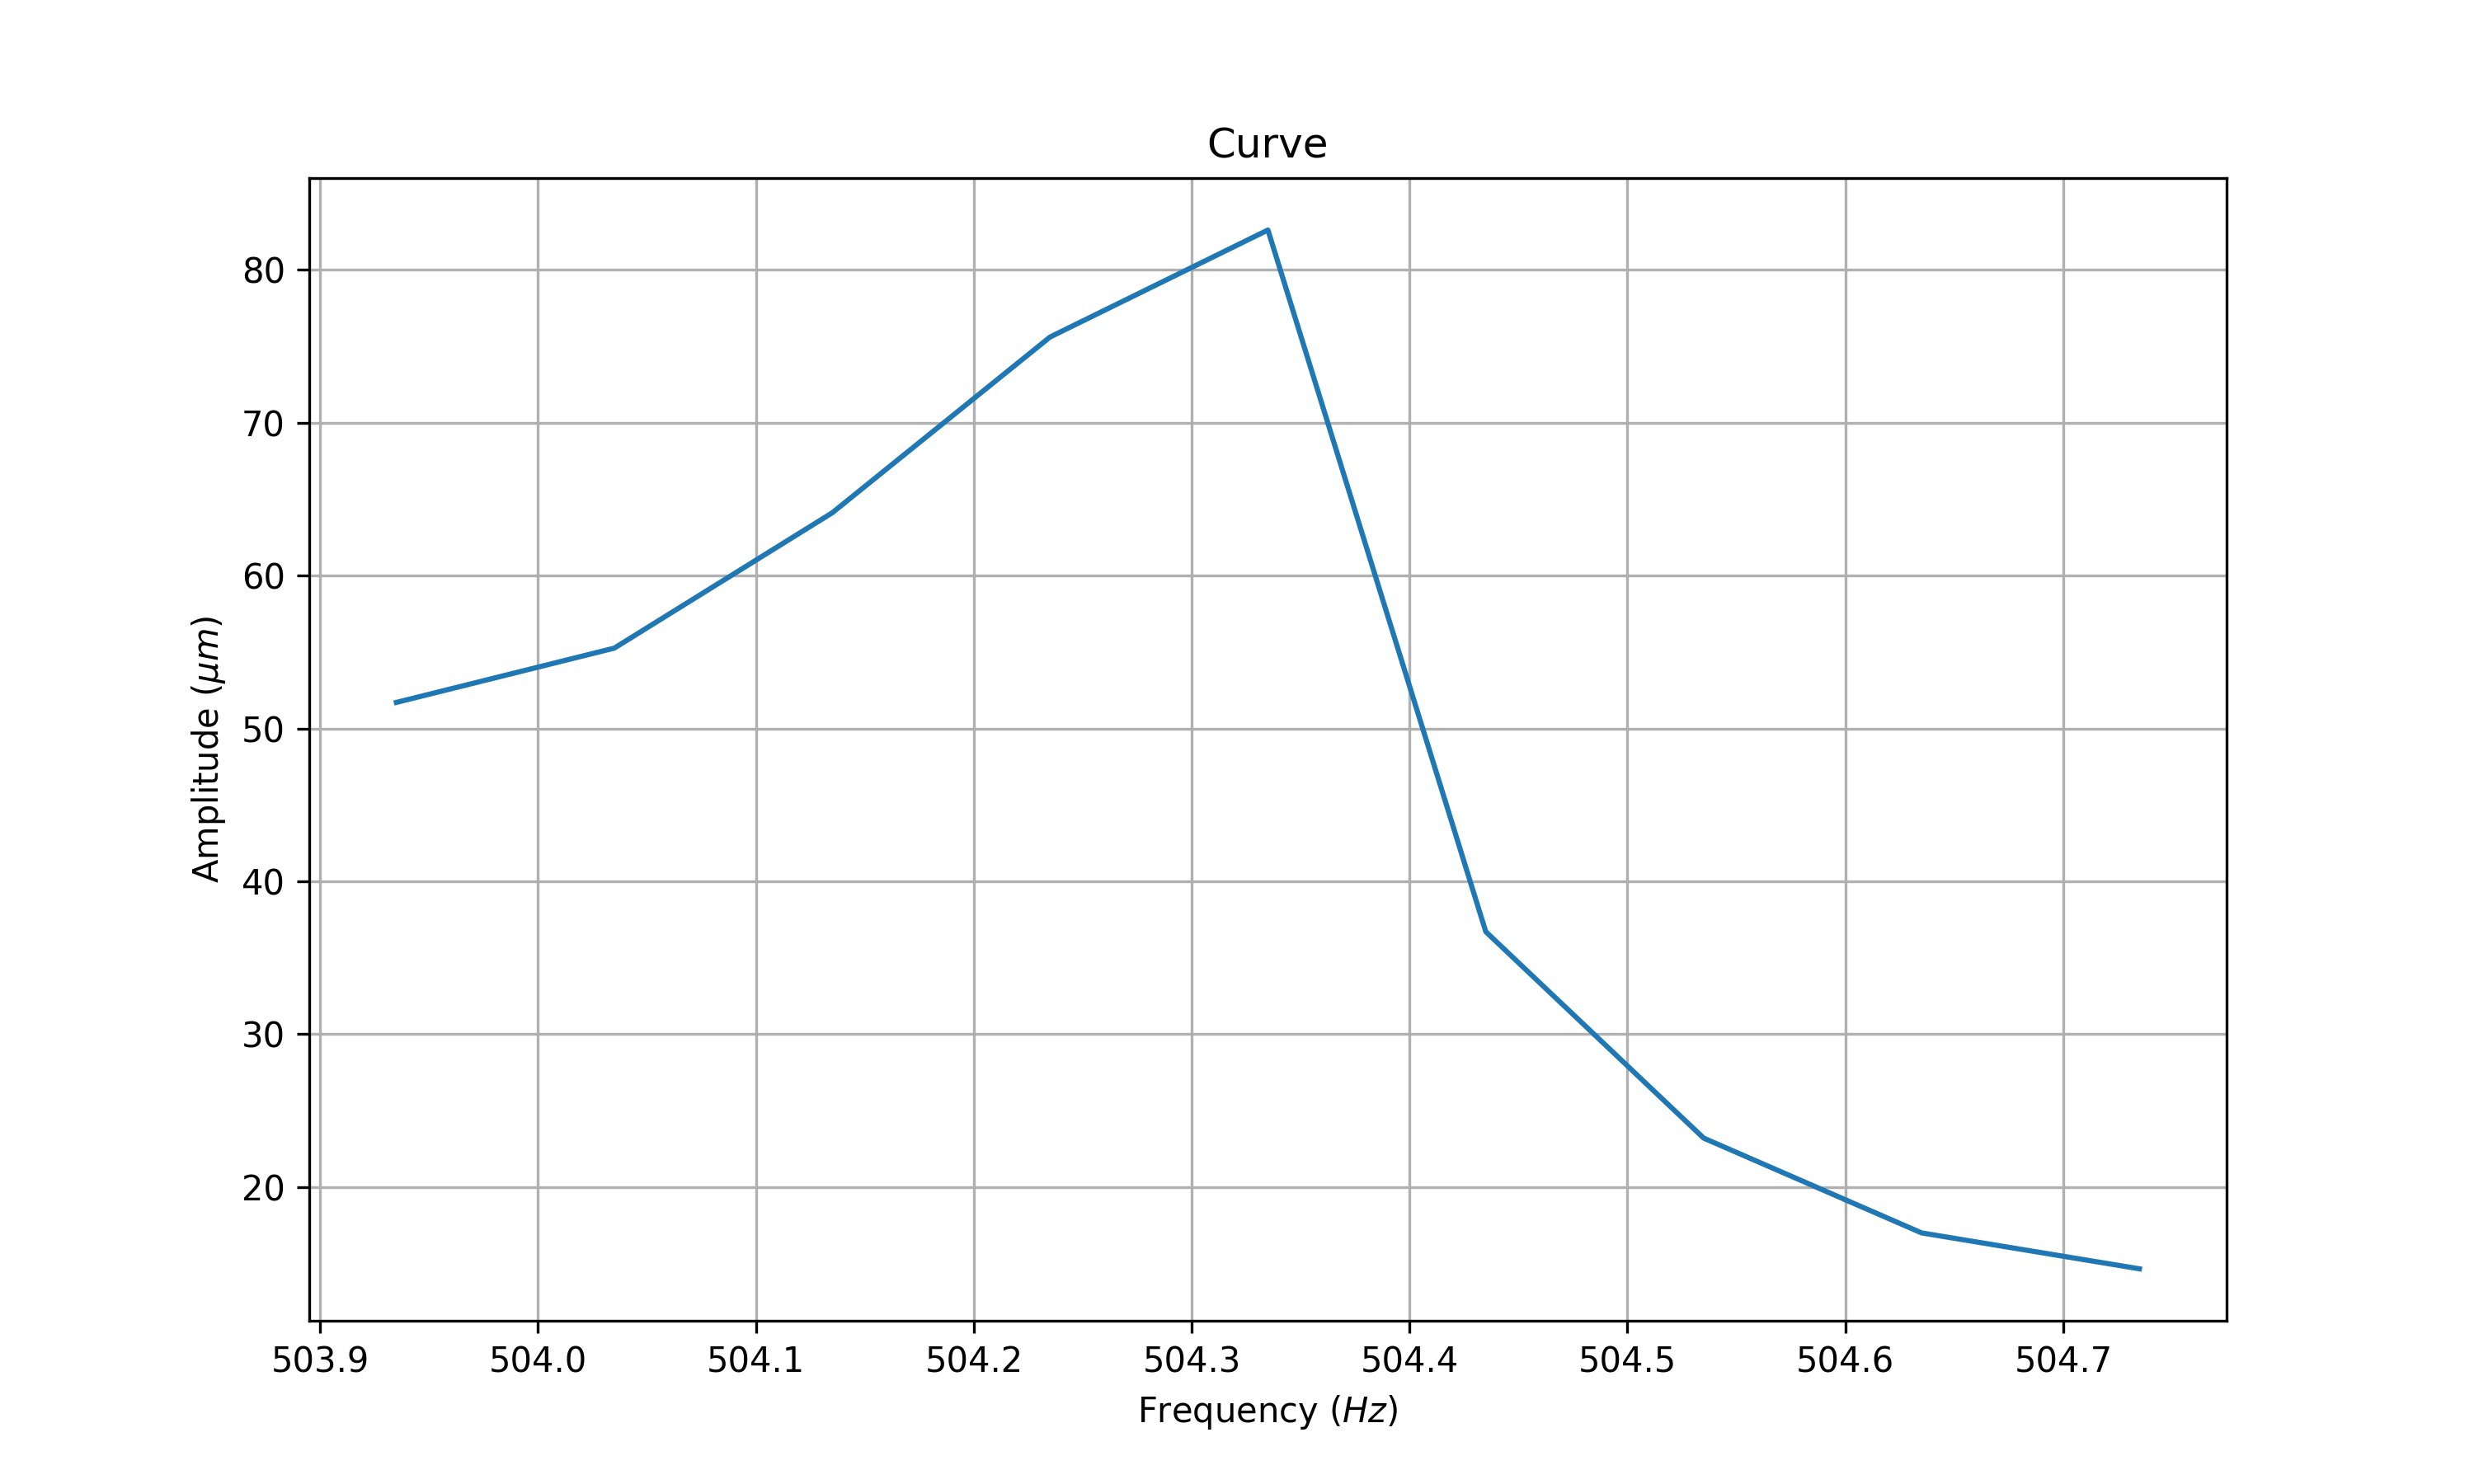
\includegraphics[width=\textwidth]{./curve.png}
    \caption{音叉振幅与驱动频率的关系曲线}
\end{figure}
\section{实验现象分析及结论}

在双光栅测量微弱振动的实验中,实验现象主要表现为音叉在不同频率下的振幅变化。首先,通过调整驱动信号的频率,测量音叉的自身固有频率,此时振幅达到最大值,示波器上显示出极多峰值,同时音叉发出人耳可听见的震动噪声。随着频率偏离固有频率,音叉的振幅逐渐减小。当驱动频率远离固有频率时,振幅显著降低,表现出典型的谐振曲线特征,即在固有频率附近振动最强,远离该频率时振动较弱。这种现象体现了音叉的共振特性和频率响应。验证了双光栅检测微弱震动的合理性。

\section{讨论题}

\subsection{测量音叉谐振曲线时,为什么要固定驱动信号功率?}

在双光栅检测微弱震动的实验中,测量音叉的谐振曲线时需要固定驱动信号功率,以确保测量结果的准确性和可靠性。首先,固定功率能够确保音叉在不同频率下受到的驱动力保持一致,从而准确反映其真实的频率响应特性。若驱动功率变化,会导致音叉振动幅度发生改变,影响谐振曲线的关键参数,如谐振频率、带宽和峰值,导致测量结果出现偏差或失真。其次,较高的功率可能引入非线性效应,使音叉表现出非线性振动行为,这会改变其正常的谐振特性。通过固定功率,可以避免过强的激励导致这些非线性现象,从而确保谐振曲线准确反映音叉的特性。此外,保持恒定的功率能够使得整个频率范围内的测量条件一致,有助于得到精确且可重复的实验结果。因此,固定驱动信号功率对于微弱振动的准确检测和分析至关重要。

\subsection{静光栅和动光栅的前后位置是否可以互换,为什么?}

在双光栅检测系统中,静光栅和动光栅的前后位置通常不可随意互换,因为它们的功能和位置在实验中扮演着不同的角色。静光栅主要用于产生参考干涉图案,提供稳定的干涉条纹作为比较基准,而动光栅用于调制光信号,反映被测物体的微弱振动。动光栅的振动会影响光束的相位,从而改变干涉条纹的相位。如果两者互换,系统将失去基于动光栅调制的检测原理。此外,光路设计也要求静光栅放置在光源前方或固定位置,以确保光束形成稳定的参考图案,而动光栅需要靠近振动源以捕捉振动信号。如果动光栅放在前面,会导致输入光场的不稳定,破坏干涉条纹的参考信号,从而影响测量的准确性。互换它们的位置还会导致干涉条纹的不稳定,使系统无法进行精确的振动检测。因此,静光栅和动光栅的位置设计是基于各自功能的互补性,互换它们将使系统失去原有的检测能力,无法有效测量微弱振动。

\end{document}